% IEEE standard conference template; to be used with:
%   spconf.sty  - LaTeX style file, and
%   IEEEbib.bst - IEEE bibliography style file.
% --------------------------------------------------------------------------

\documentclass[letterpaper]{article}
\usepackage{spconf,amsmath,amssymb,graphicx}
\usepackage[utf8]{inputenc}
\usepackage[linesnumbered, ruled]{algorithm2e}

% Example definitions.
% --------------------
% nice symbols for real and complex numbers
\newcommand{\R}[0]{\mathbb{R}}
\newcommand{\C}[0]{\mathbb{C}}

% bold paragraph titles
\newcommand{\mypar}[1]{{\bf #1.}}

% Title.
% ------
\title{A parallel implementation of the Gumtree Algorithm in C++}
%
% Single address.
% ---------------
%\name{Balz Guenat, Christopher Signer, Amirreza Bahreini}
\name{Balz Guenat, Christopher Signer}
\address{Department of Computer Science\\ ETH Zürich\\Zürich, Switzerland}

% For example:
% ------------
%\address{School\\
%		 Department\\
%		 Address}
%
% Two addresses (uncomment and modify for two-address case).
% ----------------------------------------------------------
%\twoauthors
%  {A. Author-one, B. Author-two\sthanks{Thanks to XYZ agency for funding.}}
%		 {School A-B\\
%		 Department A-B\\
%		 Address A-B}
%  {C. Author-three, D. Author-four\sthanks{The fourth author performed the work
%		 while at ...}}
%		 {School C-D\\
%		 Department C-D\\
%		 Address C-D}
%

\begin{document}
%\ninept
%
\maketitle
%

\begin{abstract}
TODO Describe in concise words what you do, why you do it (not necessarily
in this order), and the main result.  The abstract has to be
self-contained and readable for a person in the general area. You
should write the abstract last.

The evolution of software projects is recorded with version control systems which store snapshots of the project at different points in time. To help developers understand the transitions between these snapshots, \emph{diff} programs are used to highlight the differences between them. In an effort to provide developers with a better description of these differences the \emph{Gumtree} algorithm computes a matching between the nodes of the abstract syntax trees of the two snapshots.

\emph{Gumtree} is an algorithm to compute a matching between the nodes of two similar abstract syntax trees.
\end{abstract}

\section{Introduction}\label{sec:intro}

%In this section we explain the problem the \emph{Gumtree} algorithm attempts to solve and state the goal of our work.

Software projects evolve over the time of their development and operation.
Nowadays the history of such evolution is typically recorded by a version control system (VCS) which stores snapshots of the project state.
For the developers to understand this evolution, it is of tremendous help if not only these snapshots are available but also a representation of the transition from one state the other.
Often these transitions are represented in form of differences between the files or edit operations transforming the old into the new file.
The transitions are usually not stored explicitly but are computed from the two states at the user's request.
Algorithms performing this computation are called diff algorithms.
Most popular diff algorithms like \emph{diff}, \emph{kdiff3} and \emph{git-diff} regard all files as lists of lines and find the differences between them by computing their longest common subsequence.

This approach is simple and fast but it is often too coarse grained and lacks conciseness.
Consider for example the definition of a Java method that is moved from the top of a file to the bottom of the same file.
\emph{git-diff} will regard this as a deletion of multiple lines at the top of the file and an unrelated addition of multiple lines at the bottom.

The \emph{Gumtree} algorithm introduced by Falleri et al. \cite{falleri:2014:structure_diff} is a valid attempt at overcoming these issues by leveraging the structure inherent in program code.
Instead of regarding files as lists of lines, the code is parsed to yield an abstract syntax tree (AST).
Then, in a step analogous to finding the longest common subsequence of lists, a matching between the two versions of the AST is computed and finally a description of edit operations is generated.
The main contribution of the \emph{Gumtree} algorithm is a way to find said matching.
Using this structure-aware approach, the example from before will be represented as a single move operation of the AST node representing the method definition.

The disadvantages of this approach are twofold.
Firstly, it requires the integration of a parser for the respective language to generate the AST.
Secondly, parsing and subsequently finding a matching between the ASTs is much more computationally involved and thus takes a longer time.
The existing implementation written in Java \footnote{github.com/GumTreeDiff/gumtree} defers the generation of the AST to an external component but the matching itself is computed in a purely single-threaded manner.
In an attempt to alleviate the latter disadvantage, we have in a first step implemented the \emph{Gumtree} algorithm in C++ and in a second step tried to parallelize it where possible.
We will use the existing Java implementation as a reference both in terms of correctness as well as performance.

TODO: Describe what we did and what the results were.

\section{Background: The Gumtree algorithm}\label{sec:background}

This section describes the original \emph{Gumtree} algorithm as it was introduced in sections 2 and 3 in the Falleri paper \cite{falleri:2014:structure_diff}.

\mypar{Problem definition}
The \emph{Gumtree} algorithm regards ASTs as ordered rooted trees where nodes have a type and may have a string value associated to them.
%It was designed specifically with ASTs in mind but can be applied to any type of tree with these properties.
Given two such trees $T_1$ and $T_2$, the algorithm produces a matching between the nodes of the two trees.
A matching is represented as a set of pairs of nodes where each node is part of at most one pair and nodes belonging to the same pair have the same type.

\mypar{Algorithm overview}
The algorithm computes such a matching in two successive phases:
\begin{enumerate}
	\item The top-down phase in which isomorphic subtrees are found and matched.
	\item The bottom-up phase in which nodes are matched if many of their descendants have already been matched.
\end{enumerate}
The Falleri paper additionally describes the search for so-called \emph{recovery mappings} in the second phase.
We omit this step as it requires the implementation of a separate optimal algorithm which we deemed out of scope for this project.
For the purpose of comparing our implementation to the reference, we have modified the original implementation to omit this step as well.

\mypar{Top-down phase}
This phase finds and matches isomorphic subtrees down to a minimum height $minHeight$ by comparing increasingly smaller subtrees.
Unique matches are accepted immediately while subtrees that are isomorphic to multiple subtrees are matched based on the similarity of their parents at a later stage.

This phase uses a height-indexed priority list of subtrees (represented by their respective root nodes) for each tree supporting the following operations:
\emph{peekMax} returns the maximum subtree height in the list.
\emph{pop} returns the set of subtrees with maximum height and removes them from the list.
\emph{push} inserts a subtree into the list.
\emph{open} inserts all children of a node into the list.

Further we define a similarity function $sim$ on subtrees given a mapping $M$ as follows:
$$ sim(t_1, t_2, M) = \frac{| \{ t_x \in d(t_1), t_y \in d(t_2) : (t_x, t_y) \in M \} | }{ (|d(t_1)| + |d(t_2)|) / 2} $$
where $d(t)$ is the set of descendants of $t$. $sim$ rates the similarity of two subtrees in the range $[0,1]$ where a value of 1 indicates that the two nodes have the same descendants.
When a given node can be matched to multiple nodes we use this similarity measure on the parents of the candidates to decide between them.

See Algorithm \ref{alg:top-down} for a full description of the top-down phase.

\SetKw{KwOr}{or}
\SetAlFnt{\footnotesize}
\SetInd{0.3em}{0.6em}
\SetAlgoVlined

\begin{algorithm}
	\KwData{Two trees $T_1, T_2$, a minimum height $minHeight$, two empty height-indexed priority lists $L_1, L_2$, an empty list of candidate mappings $A$ and an empty set of mappings $M$}
	\KwResult{The set of mappings $M$}
	push(root($T_1$), $L_1$)\;
	push(root($T_2$), $L_2$)\;
	\While{$ min(peekMax(L_1),peekMax(L_2)) > minHeight $}{
		\eIf{$ peekMax(L_1) \neq peekMax(L_2) $}{
			\eIf{$ peekMax(L_1) > peekMax(L_2) $}{
				\lForEach{$ t \in pop(L_1) $}{
					$open(t,L_1)$
					}
				}{
				\lForEach{$ t \in pop(L_2) $}{
					$open(t,L_2)$
					}
				}
		}{
			$H_1 \gets pop(L_1)$\;
			$H_2 \gets pop(L_2)$\;
			\ForEach{$ (t_1,t_2) \in H_1 \times H_2 $}{
				\If{$ \text{isomorphic}(t_1,t_2) $}{
					\eIf{$ \exists t_y \in T_2 : \text{isomorphic}(t_1,t_y) \wedge t_y \neq t_2 $\\ \KwOr $ \exists t_x \in T_1 : \text{isomorphic}(t_x,t_2) \wedge t_x \neq t_1 $\\}{
						add($A, (t_1,t_2)$)\;
					}{
						add all pairs of isomorphic nodes of $d(t_1)$ and $d(t_2)$ to $M$\;
					}
				}{
				}
			}
			\lForEach{$ t_1 \in H_1 : (t_1,t_y) \notin A \cup M $}{$ \text{open}(t_1,L_1) $}
			\lForEach{$ t_2 \in H_2 : (t_x,t_2) \notin A \cup M $}{$ \text{open}(t_2,L_2) $}
		}
	}
	sort $(t_1,t_2) \in A$ using $sim(parent(t_1),parent(t_2), M)$\;
	\While{$\text{size}(A) > 0$}{
		$(t_1,t_2) \gets \text{popLargest}(A)$\;
		add all pairs of isomorphic nodes of $d(t_1)$ and $d(t_2)$ to $M$\;
		$A \gets A \setminus \{(t_1,t_y) \in A\}$\;
		$A \gets A \setminus \{(t_x,t_2) \in A\}$\;
	}
\caption{The top-down phase (taken from \cite{falleri:2014:structure_diff})}
\label{alg:top-down}
\end{algorithm}

\mypar{Bottom-up phase}
The bottom-up phase takes the mappings computed by the top-down phase as input.
$T_1$ is traversed in post-order and for each non-leaf node $t_1$ that has not been matched yet, a list of candidate nodes from $T_2$ is computed.
A node $c \in T_2$ is a candidate for $t_1$ if it is unmatched, has the same type as $t_1$ and has some matching descendants.
$t_1$ is then matched with the candidate with the largest similarity value $sim(t_1,c,M)$ provided it is over a certain threshold $minSim$.

See Algorithm \ref{alg:bottom-up} for a full description of the top-down phase.
The mapping $M$ resulting from this phase is the final output of the \emph{Gumtree} algorithm without \emph{recovery mappings}.

\begin{algorithm}
	\KwData{Two trees $T_1, T_2$, a set of mappings $M$ (from the top-down phase) and a threshold $minSim$}
	\KwResult{The set of mappings $M$}
	\ForEach{$t_1 \in T_1$ in post-order}{
		\If{$t_1$ is not matched $\wedge t_1$ has matched children}{
			$t_2 \gets \text{bestCandidate}(t_1,M)$\;
			\If{$ t_2 \neq null \wedge sim(t_1,t_2,M) > minSim $}{
				add $(t_1,t_2)$ to $M$\;
			}
		}
	}
\caption{The bottom-up phase (without \emph{recovery mappings})}
\label{alg:bottom-up}
\end{algorithm}

\mypar{Chosen thresholds}
We set the named thresholds to $minSim=0.5$ and $minheight=2$ as recommended in the Falleri paper \cite{falleri:2014:structure_diff}.

\section{Parallel implementation in C++}\label{sec:yourmethod}

In this section we present our implementation of the \emph{Gumtree} algorithm written in C++ and describe our efforts to parallelize it.
To achieve parallelization, we make use of the OpenMP API\footnote{openmp.org}.
The entire project is open source and available on Github\footnote{github.com/BalzGuenat/ParallelGumtree}.

\mypar{Existing Java implementation}
The authors of the original paper provide an implementation written in Java which is publicly available on Github\footnote{github.com/GumTreeDiff/gumtree}.
%The back-end of this implementation is built in a modular fashion so as to support the easy integration of different 

\mypar{Writing Gumtree in C++}
To write our implementation we adhered very closely to the existing Java implementation.
We specify a simple encoding format for the input trees.
TODO: explain encoding?
Two files each representing one input tree are read, parsed and the trees are constructed.

\mypar{Finding potential for parallel execution}

TODO: Explain where we saw potential for parallelization and why some parts are not (easily) parallelizable.

We examined the algorithm with the goal of finding sections that could easily be parallelized.

\mypar{Checking for isomorphism}
Checking if two subtrees are isomorphic is an operation that occurs often in the top-down phase.
Further, it is a read-only operation which facilitates parallel execution.
To check if two subtrees are isomorphic we first check whether their respective root nodes have the same type and the same number of children.
If yes, we iterate over their children and for each child pair, we create an OpenMP task that recursively checks if the pair is isomorphic.
To avoid unnecessary overhead, we only execute the check in parallel if the size of the subtree is above a certain threshold \emph{SubtreeSizeCutoff}.
The size of a subtree is the total number of nodes in that subtree.

\mypar{Finding the best candidate}
In the bottom-up phase on line 3 we search for the best candidate to match with a given node $t_1$.
Remember that a node $c \in T_2$ is a candidate for $t_1$ if it is unmatched, has the same type as $t_1$ and has some matching descendants.
The best candidate is the one with the largest similarity value $sim(t_1,c,M)$.
%We parallelize the search for the best candidate by distributing the 
We first gather all candidates in a list and then use the OpenMP parallel for-loop pragma to distribute the search for the best candidate over multiple threads.
To avoid unnecessary overhead, we only execute the search in parallel if the number of candidates is greater than a certain threshold \emph{CandidatesSizeCutoff}.
%In the top-down phase on line 12, we iterate over the cross product of two potentially large

\section{Randomized test case generation}

In order to test and evaluate our implementation we need test cases large enough for the execution time to be an inconvenience for the user i.e. multiple seconds.
We chose to implement a tree generator that randomly generates trees in the following fashion.
TODO: Explain random tree generator

\section{Experimental Results}\label{sec:exp}

In this section we describe the setup we used to run performance tests, report the measurements made and present our interpretation of them.

\mypar{Experimental setup}
To compile the project we use GCC 5.2.1 with the \texttt{-O2} optimization level.
We run our performance tests in Ubuntu 15.10 running on an Intel Core i7-3520M running at 2.9GHz with 4 logical cores on 2 physical cores.
The system has 8GB of memory.
The Java reference implementation is run in the OpenJDK Runtime Environment 1.8.0.
We believe this system is a typical environment in which \emph{diff} programs such as \emph{Gumtree} are run in.

For each approximate tree size, we generate several different test cases and then measure the time the different implementations take to produce a result.

\mypar{Results}
First, we compare our implementation to the Java reference implementation.
Figure \ref{fig:cpp_vs_java} shows the execution time of the implementations with various input sizes.
The input size is the average number of nodes in the two input trees.
We see that especially for smaller input sizes, the C++ implementation is faster than the reference implementation.

We then examine how well our implementation scales when executed with multiple threads.
Figure \ref{fig:cpp_speedup} shows the speedup achieved with 2 and 4 threads with various input sizes.
We see that our implementation hardly ever achieves a speedup of over 1 and thus does not benefit at all from running on multiple threads.

\mypar{Possible reasons for bad scaling}
We further examine our implementation 

\begin{figure}
	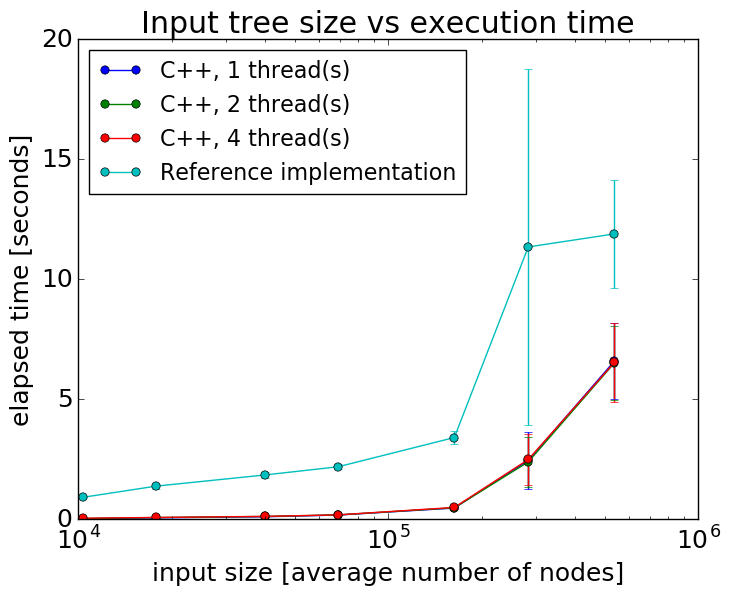
\includegraphics[width=\linewidth]{timePlot_with_java}
	\label{fig:cpp_vs_java}
	\caption{Execution time of the different implementations with various input sizes and 10 different randomly generated test cases for each input size. The bars show the standard deviation of the individual test cases from the mean execution time for that input size.}
\end{figure}

\begin{figure}
	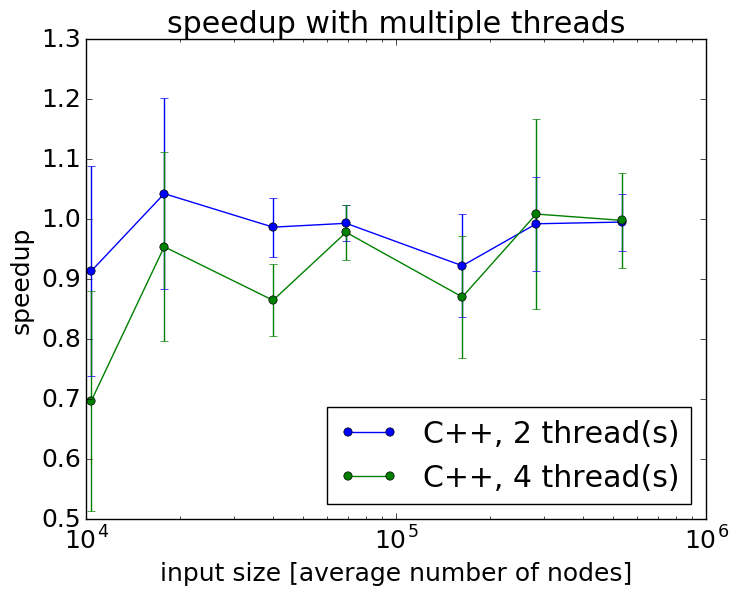
\includegraphics[width=\linewidth]{speedupPlot_with_java}
	\label{fig:cpp_speedup}
	\caption{Speedup compared to single threaded execution with various input sizes and 10 different randomly generated test cases for each input size. The bars show the standard deviation of the individual test cases from the mean speedup for that input size.}
\end{figure}

Here you evaluate your work using experiments. You start again with a
very short summary of the section. The typical structure follows.

\mypar{Experimental setup} Specify the platform (processor, frequency, maybe OS, maybe cache sizes)
as well as the compiler, version, and flags used. If your work is about performance, 
I strongly recommend that you play with optimization flags and consider also icc for additional potential speedup.

Then explain what kind of benchmarks you ran. The idea is to give enough information so the experiments are reproducible by somebody else on his or her code.
For sorting you would talk about the input sizes. For a tool that performs NUMA optimization, you would specify the programs you ran.

\mypar{Results}
Next divide the experiments into classes, one paragraph for each. In each class of experiments you typically pursue one questions that then is answered by a suitable plot or plots. For example, first you may want to investigate the performance behavior with changing input size, then how your code compares to external benchmarks.

For some tips on benchmarking including how to create a decent viewgraph see pages 22--27 in \cite{Pueschel:10}.

{\bf Comments:}
\begin{itemize}
\item Create very readable, attractive plots (do 1 column, not 2 column plots
for this report) with readable font size. However, the font size should also not be too large; typically it is smaller than the text font size.
An example is in Fig.~\ref{fftperf} (of course you can have a different style).
\item Every plot answers a question. You state this question and extract the
answer from the plot in its discussion.
\item Every plot should be referenced and discussed.
\end{itemize}

\begin{figure}\centering
  \caption{Performance of four single precision implementations of the
  discrete Fourier transform. The operations count is roughly the
  same. The labels in this plot are maybe a little bit too small.\label{fftperf}}
\end{figure}

\section{Conclusions}

In a first step we have implemented the \emph{Gumtree} algorithm in C++.
We then found several sections in the algorithm that could be parallelized and used OpenMP to implement these parallelizations.
To test and evaluate our implementation we needed pairs of trees large enough so we implemented a randomized tree generator to create these test cases.
Our performance tests with randomly generated trees showed that while our implementation runs faster than the Java reference implementation, it does not scale with multiple threads.
We noticed that the proportion of execution time spent in parallel sections can heavily depend on the problem instance.
This made us doubt the validity of the problem instances that we randomly generate in the sense that they do not resemble real changes made to ASTs closely enough.
It is possible that the generated test cases tend to result in problem instances where only a small proportion of the time is spent in parallel sections.
To eliminate the possibility of invalid test cases we used \emph{clang} to parse real software projects and dump their ASTs.
We then converted these ASTs to our encoding format and used the so created test cases to evaluate the performance of the two implementations and their scaling behavior.

Here you need to summarize what you did and why this is
important. {\em Do not take the abstract} and put it in the past
tense. Remember, now the reader has (hopefully) read the report, so it
is a very different situation from the abstract. Try to highlight
important results and say the things you really want to get across
such as high-level statements (e.g., we believe that .... is the right
approach to .... Even though we only considered x, the
.... technique should be applicable ....) You can also formulate next
steps if you want. Be brief. After the conclusions there are only the references.

\section{Further comments}

Here we provide some further tips.

\mypar{Further general guidelines}

\begin{itemize}
\item For short papers, to save space, I use paragraph titles instead of
subsections, as shown in the introduction.

\item It is generally a good idea to break sections into such smaller
units for readability and since it helps you to (visually) structure the story.

\item The above section titles should be adapted to more precisely
reflect what you do.

\item Each section should be started with a very
short summary of what the reader can expect in this section. Nothing
more awkward as when the story starts and one does not know what the
direction is or the goal.

\item Make sure you define every acronym you use, no matter how
convinced you are the reader knows it.

\item Always spell-check before you submit (to us in this case).

\item Be picky. When writing a paper you should always strive for very
high quality. Many people may read it and the quality makes a big difference.
In this class, the quality is part of the grade.

\item Books helping you to write better: \cite{Higham:98} and \cite{Strunk:00}.

\item Conversion to pdf (latex users only): 

dvips -o conference.ps -t letter -Ppdf -G0 conference.dvi

and then

ps2pdf conference.ps
\end{itemize}

\mypar{Graphics} For plots that are not images {\em never} generate the bitmap formats
jpeg, gif, bmp, tif. Use eps, which means encapsulate postscript. It is
scalable since it is a vector graphic description of your graph. E.g.,
from Matlab, you can export to eps.

The format pdf is also fine for plots (you need pdflatex then), but only if the plot was never before in the format 
jpeg, gif, bmp, tif.


% References should be produced using the bibtex program from suitable
% BiBTeX files (here: bibl_conf). The IEEEbib.bst bibliography
% style file from IEEE produces unsorted bibliography list.
% -------------------------------------------------------------------------
\bibliographystyle{IEEEbib}
\bibliography{bibl_conf}

\end{document}

